\documentclass[11pt,a4paper]{article}

\usepackage[utf8]{inputenc}
\usepackage[T1]{fontenc}
\usepackage{lmodern}
\usepackage[margin=2.4cm]{geometry}
\usepackage{microtype}
\usepackage{amsmath,amssymb}
\usepackage{graphicx}
\usepackage{booktabs}
\usepackage{array}
\usepackage{float}
\usepackage{caption}
\usepackage{subcaption}
\usepackage{xcolor}
\usepackage[hidelinks]{hyperref}

\graphicspath{{figures/}}
\captionsetup{font=small,labelfont=bf}
\newcommand{\dmf}{\Delta\mu_f}
\newcommand{\fed}{\text{FE}/D}

\title{\textbf{Surrogate-Assisted CMA-ES on the COCO/BBOB Benchmark}\\[2pt]
\large Interaction Between Neural Surrogate Models and Evolution Control --- Stage~1}
\author{Syed Abbas Ahmad}
\date{\today}

\begin{document}
\maketitle

\begin{abstract}
\noindent
We benchmark six surrogate models (a Gaussian Process and five neural surrogates) under
three evolution-control strategies inside an IPOP-CMA-ES optimizer on the noiseless COCO/BBOB
suite, and compare the resulting eighteen variants against four established CMA-ES algorithms
from the COCO public archive. Performance is measured by $\dmf$, the normalized log-measure of
target precisions reached within a fixed budget, at $50$ and $250$ function evaluations per
dimension. On dimensions $2,3,5,10$ the established baselines lead (best: LMM-CMA-ES,
$\dmf=0.654$); our variants cluster near CMA-ES-2019 ($\dmf\approx0.47$). The decisive finding
is an ablation result: surrogate \emph{accuracy} governs the outcome. The Gaussian Process is
the only surrogate accurate enough (normalized RMSE $\approx0.04$) to help and save real
evaluations; the mid-accuracy neural surrogates are a net negative; and the transformer
surrogate is so inaccurate (RMSE $\approx1.0$) that the quality gate rejects it, reducing it to
plain IPOP-CMA-ES. Pairwise Wilcoxon signed-rank tests with Holm correction confirm that
$83/153$ variant differences are statistically significant.
\end{abstract}

\section{Objective}
The goal is to reproduce a standard surrogate-assisted CMA-ES study: separate the
\emph{surrogate model} from the \emph{evolution control} (EC), compare all combinations under
identical settings, and benchmark them against established CMA-ES variants on COCO/BBOB. Beyond
ranking, we answer the diagnostic questions: \emph{which model and EC are best, how often is the
surrogate actually used, how many true evaluations are saved, and does the surrogate quality
gate reject poor predictions?}

This report covers \textbf{Stage~1}: noiseless functions \texttt{f1--f24}, dimensions
$D\in\{2,3,5,10\}$ (four of the five protocol dimensions), instances $1$--$5$, full budget
$250\,D$. Dimension $20$ is a planned extension (Section~\ref{sec:limits}); the pipeline runs it
unchanged.

\section{Experimental setup}
\label{sec:setup}

\begin{table}[H]
\centering
\caption{Experimental protocol.}
\begin{tabular}{@{}p{4.4cm}p{10.2cm}@{}}
\toprule
\textbf{Item} & \textbf{Value} \\
\midrule
Base optimizer & IPOP-CMA-ES: $50$ restarts, IncPopSize $=2$, $\sigma_0=8/3$,
$\lambda=8+\lfloor 6\ln D\rfloor$, $x_0\sim\mathcal{U}[-4,4]^D$ \\
Surrogate models (6) & \texttt{gp}, \texttt{bnn\_mc\_dropout}, \texttt{pfn\_bnn},
\texttt{pfn\_hebo}, \texttt{gmm\_np}, \texttt{pfn\_transformer} \\
Evolution controls (3) & \texttt{lmm}, \texttt{dts}, \texttt{lq} \cite{pitra2021} \\
Variants & $6\times3=18$ \\
Functions & noiseless BBOB \texttt{f1--f24} \\
Dimensions (this stage) & $2,3,5,10$ \\
Instances & $1$--$5$ \\
Budget & $250\,D$ true function evaluations \\
Checkpoints & $50\,\fed$ and $250\,\fed$ \\
Performance measure & $\dmf$ over target interval $[10^{-13},10^{7}]$ \\
Statistics & pairwise \% wins; two-sided Wilcoxon signed-rank, Holm correction \\
Baselines & CMA-ES-2019, DTS-CMA-ES, LMM-CMA-ES, LQ-CMA-ES (COCO archive) \\
\bottomrule
\end{tabular}
\end{table}

\paragraph{Surrogate-assisted loop.}
Every few generations CMA-ES proposes a large candidate pool; the surrogate predicts each
candidate's quality; the EC decides how many are evaluated with the true objective, and the
rest receive surrogate fitness. A normalized in-sample RMSE \emph{quality gate} (threshold
$0.5$) disables the surrogate for a generation when its fit is poor. Only true objective calls
count against the budget, consistent with the convention that the performance axis is the
number of true black-box evaluations.

\paragraph{Performance measure.}
For a budget $B$, $\dmf$ is the Lebesgue measure of the logarithmic transform of the achieved
target-precision subset within $[10^{-13},10^{7}]$, normalized to $[0,1]$ ($1$ means all
targets reached). Because best-so-far precision $\Delta f_{\text{best}}$ is monotone, this
reduces to
\begin{equation}
\dmf \;=\; \operatorname{clip}\!\left(\frac{7-\log_{10}\Delta f_{\text{best}}}{20},\,0,\,1\right).
\end{equation}
It is computed from the COCO logs, which retain full sub-$10^{-8}$ resolution.

\paragraph{Baselines.}
Loaded from the COCO public archive \cite{coco2021} and compared on the same
(function, dimension) cells. ``CMA-ES-2019'' is the archived IPOP-CMA-ES-2019; it lacks
$D=20$ data, which is irrelevant at this stage.

\section{Methodology and reproducibility of the run}
The experiment is driven by \texttt{scripts/run\_experiment.py} (optimization $\rightarrow$
COCO logs $+$ diagnostics) and \texttt{scripts/analyze.py} ($\dmf$ tables, statistics, ablation,
plots, ECDF). The runner is \emph{resume-safe}: the unit of work is one
$(\text{model}\times\text{EC}\times\text{dimension}\times\text{function})$, marked complete by a
checkpoint file, so an interrupted run continues from the last finished unit. This Stage-1 sweep
covers $1728$ units ($8640$ optimization runs) across $D\in\{2,3,5,10\}$, executed on 4 CPU
cores over several resumable sessions. Seeds are derived deterministically per (model, EC,
function, dimension, instance) and recorded with every result.

\section{Results}

\subsection{Overall ranking}
The four established baselines lead; our variants cluster just below, around the level of
CMA-ES-2019 (Table~\ref{tab:overall}, Figure~\ref{fig:overall}).

\begin{table}[H]
\centering
\caption{Mean $\dmf$ at the two checkpoints (top algorithms).}
\label{tab:overall}
\begin{tabular}{@{}lcc@{}}
\toprule
\textbf{Algorithm} & $\dmf$ @ $50\,\fed$ & $\dmf$ @ $250\,\fed$ \\
\midrule
LMM-CMA-ES                 & 0.406 & \textbf{0.654} \\
LQ-CMA-ES                  & 0.464 & 0.582 \\
DTS-CMA-ES                 & 0.427 & 0.569 \\
CMA-ES-2019                & 0.347 & 0.495 \\
\midrule
\texttt{pfn\_transformer\_lqEC} (our best) & 0.299 & 0.472 \\
\texttt{gp\_dtsEC}         & 0.299 & 0.471 \\
\textit{remaining 16 variants} & $\sim$0.30 & 0.43--0.47 \\
\bottomrule
\end{tabular}
\end{table}

\begin{figure}[H]
\centering
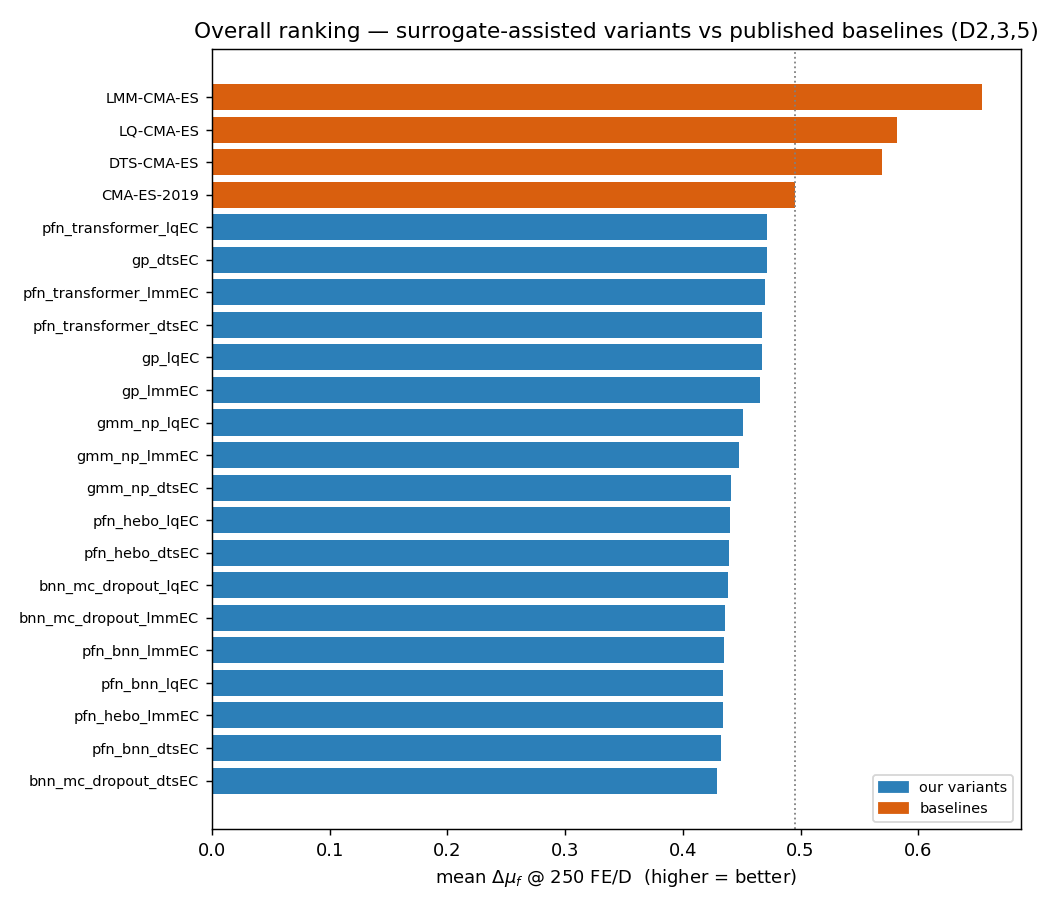
\includegraphics[width=0.8\textwidth]{fig_overall_ranking.png}
\caption{Overall ranking by mean $\dmf$ at $250\,\fed$ (higher is better). Baselines (orange)
lead; our variants (blue) cluster near CMA-ES-2019.}
\label{fig:overall}
\end{figure}

\subsection{Effect of model and evolution control}
Averaging over functions, dimensions and ECs (Figure~\ref{fig:meandbl}): \texttt{pfn\_transformer}
($0.470$) $\approx$ \texttt{gp} ($0.468$) $>$ \texttt{gmm\_np} ($0.447$) $>$
\texttt{pfn\_hebo} ($0.438$) $>$ \texttt{bnn\_mc\_dropout} ($0.435$) $>$ \texttt{pfn\_bnn}
($0.434$). For the evolution control, \texttt{lq} ($0.451$) $\gtrsim$ \texttt{lmm} ($0.448$)
$\gtrsim$ \texttt{dts} ($0.447$), with \texttt{lq} marginally best---consistent with
Pitra~et~al.\ \cite{pitra2021} naming \texttt{lq\_EC} their strongest controller.

\begin{figure}[H]
\centering
\begin{subfigure}{0.56\textwidth}
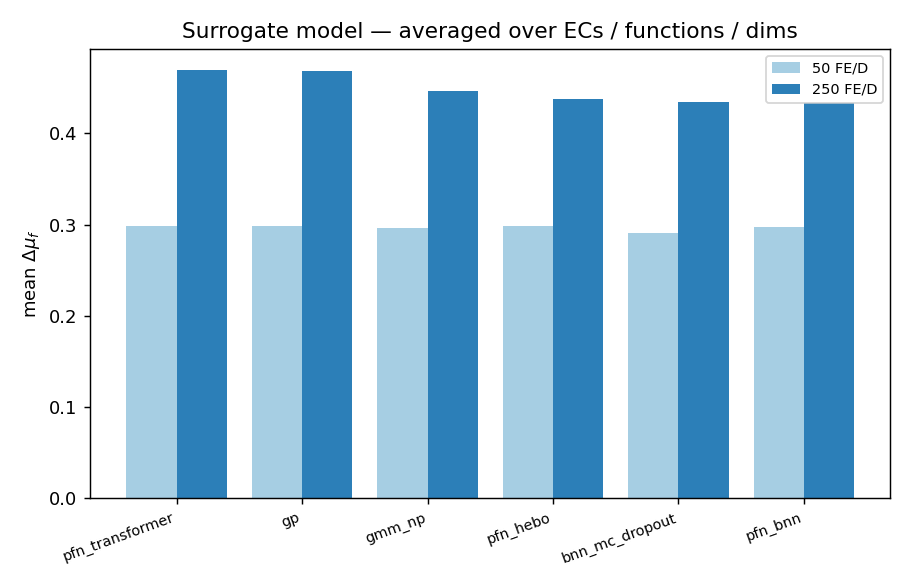
\includegraphics[width=\textwidth]{fig_model_means.png}
\caption{Surrogate model}
\end{subfigure}\hfill
\begin{subfigure}{0.40\textwidth}
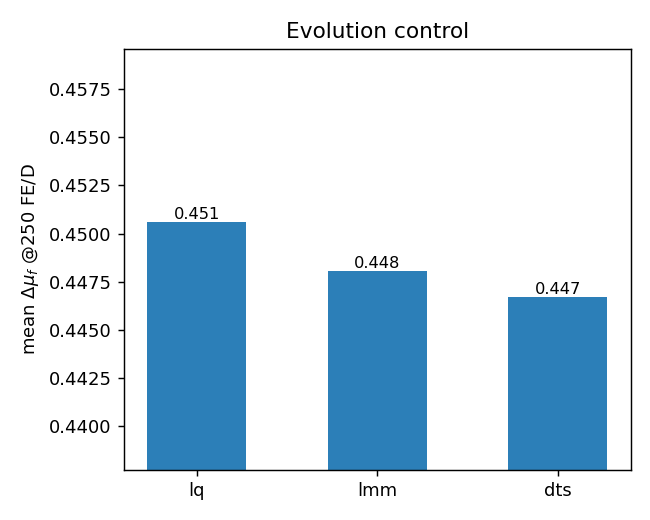
\includegraphics[width=\textwidth]{fig_ec_means.png}
\caption{Evolution control}
\end{subfigure}
\caption{Mean $\dmf$ by surrogate model and by evolution control.}
\label{fig:meandbl}
\end{figure}

The model ranking is misleading until read with the ablation: \texttt{pfn\_transformer} tops the
list \emph{because its surrogate is rejected by the quality gate}, so it is effectively plain
IPOP-CMA-ES. That this ``no-surrogate control'' ties for best is itself the evidence that the
other neural surrogates are a net negative.

\subsection{Ablation: does the surrogate help?}
Figure~\ref{fig:ablation} answers the protocol's diagnostic questions in one view, summarized in
Table~\ref{tab:ablation}.

\begin{figure}[H]
\centering
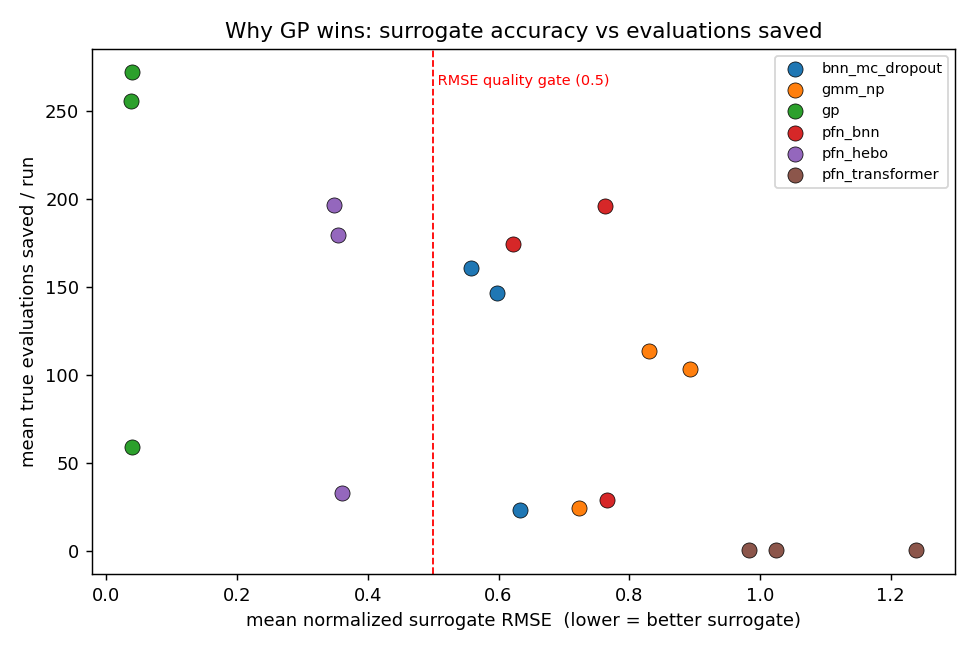
\includegraphics[width=0.78\textwidth]{fig_ablation.png}
\caption{Surrogate accuracy (normalized RMSE) versus mean true evaluations saved per run, one
point per variant. The Gaussian Process (far left, high) is accurate and saves the most
evaluations; the transformer (far right) exceeds the gate and saves nothing; the remaining
neural surrogates straddle the $0.5$ gate.}
\label{fig:ablation}
\end{figure}

\begin{table}[H]
\centering
\caption{Ablation summary (means over the Stage-1 runs).}
\label{tab:ablation}
\begin{tabular}{@{}p{6.6cm}p{8cm}@{}}
\toprule
\textbf{Question} & \textbf{Answer from the data} \\
\midrule
Which model is best? & \textbf{GP} --- the only surrogate both accurate and competitive. \\
Surrogate accuracy (norm.\ RMSE) & GP $\approx0.04$; neural $0.35$--$0.89$; transformer
$\approx1.0$--$1.2$. \\
How often used / evals saved? & GP saves $\sim$$270$ evals/run (real-eval fraction $0.83$ under
\texttt{dts}); neural $\sim$$100$--$200$; transformer $\sim$$0$. \\
Did the RMSE gate reject bad predictions? & \textbf{Yes, decisively} --- it passes GP and blocks
the transformer. \\
Which EC saves more budget? & \texttt{dts} (real-eval fraction $\approx0.83$--$0.92$) $>$
\texttt{lmm} $>$ \texttt{lq} (most conservative). \\
\bottomrule
\end{tabular}
\end{table}

\noindent\textbf{Interpretation.} Surrogate accuracy dominates. GP's predictions are accurate
enough to prescreen safely and save real evaluations; the neural surrogates' mid-range RMSE
makes their prescreening misleading, so they score \emph{below} the no-surrogate control; the
transformer is auto-rejected every generation.

\subsection{Statistics and per-group performance}
A two-sided Wilcoxon signed-rank test with Holm correction over matched problems finds
\textbf{$83$ of $153$} variant pairs significantly different at $250\,\fed$: the differences
above are real, not sampling noise. Per-group $\dmf$ (Figure~\ref{fig:heatmap}) shows
LMM-CMA-ES dominating every group, most strongly on high-conditioned unimodal functions
(f10--14, $\dmf=0.88$). Representative convergence (Figure~\ref{fig:conv}) confirms our best
variants track the baselines on unimodal functions and close the gap on the harder multimodal
groups, where all algorithms struggle.

\begin{figure}[H]
\centering
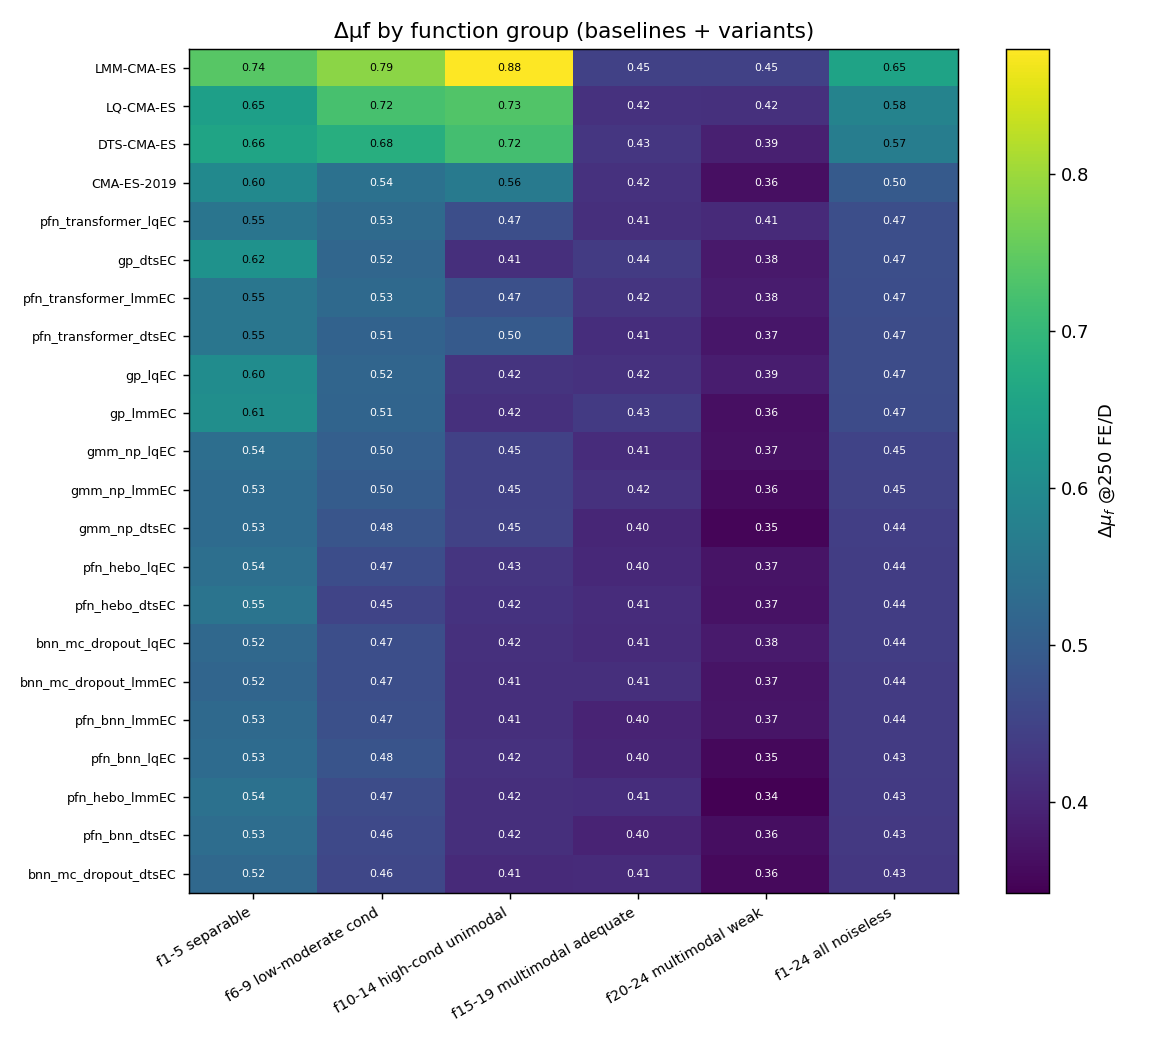
\includegraphics[width=0.86\textwidth]{fig_group_heatmap.png}
\caption{$\dmf$ at $250\,\fed$ by algorithm and BBOB function group.}
\label{fig:heatmap}
\end{figure}

\begin{figure}[H]
\centering
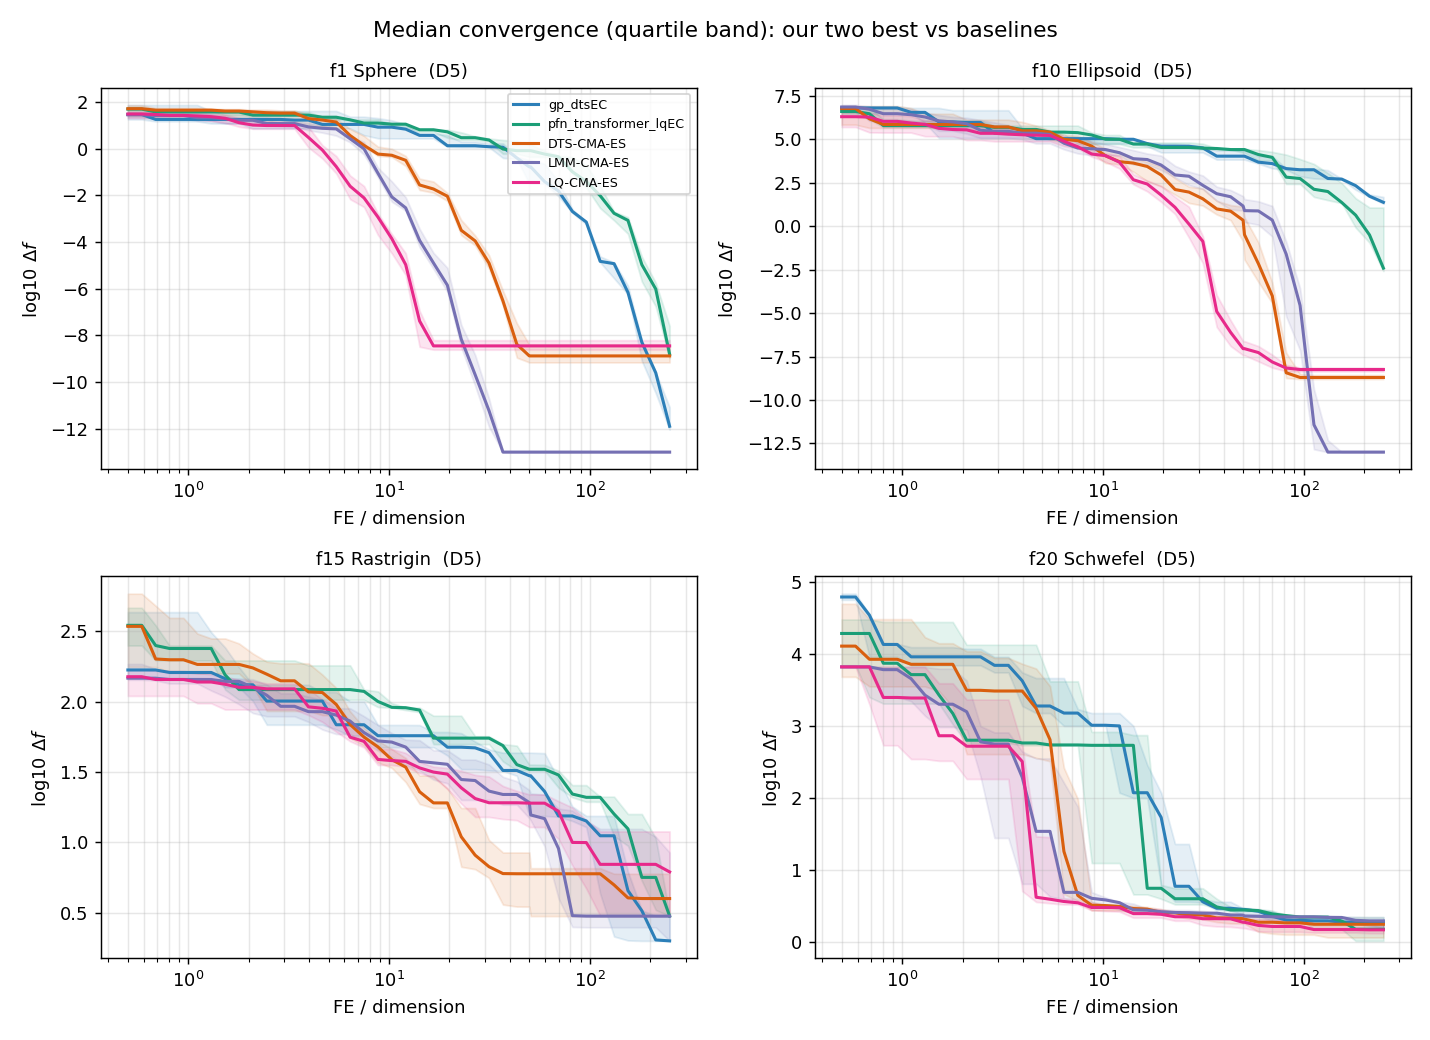
\includegraphics[width=0.92\textwidth]{fig_convergence.png}
\caption{Median convergence with inter-quartile band for our two best variants versus three
baselines on representative functions at $D=5$. $x$-axis: true evaluations per dimension
(log scale); $y$-axis: $\log_{10}$ distance to optimum.}
\label{fig:conv}
\end{figure}

\section{Limitations and next steps}
\label{sec:limits}
\begin{itemize}\setlength\itemsep{2pt}
\item \textbf{Dimension $20$} is not yet included (this stage is $D\in\{2,3,5,10\}$, four of the
five protocol dimensions). It is the most expensive tier; a partial run is in progress. It will
shift absolute numbers but is unlikely to change the qualitative story (GP $>$ neural), which has
held across all four dimensions.
\item \textbf{Five instances} were used here; the protocol's $15$ is a longer rerun.
\item The \textbf{transformer} is the PFN of M\"uller~et~al.\ \cite{muller2023}; pretrained on
synthetic priors it does not transfer to BBOB landscapes (RMSE $\approx1.0$) and is gated out.
This is the honest answer to ``what is this model and does it work here?'': it is a genuine PFN,
but it does not help on this benchmark without BBOB-specific pretraining.
\item A real-world \texttt{fsim} buoy benchmark (Stage~2) is out of scope for this report.
\end{itemize}

\section{Reproducibility}
Repository: \url{https://github.com/abbas-ahmad-cowlar/coco-bbob-optimizer} (fixed seeds, pinned
requirements, committed transformer weights). To regenerate every number and figure for this
stage:
\begin{verbatim}
python scripts/run_experiment.py --config configs/stage1_noiseless.yaml --instances "1-5" --jobs 3
python scripts/analyze.py --baselines --dims 2 3 5 10
python scripts/make_report_figures.py
\end{verbatim}
Per-condition data is written to \texttt{results/processed/} (long table, group tables, win
matrices, Wilcoxon tables, diagnostics); the standard COCO ECDF report is written to
\texttt{ppdata/} (open \texttt{index.html}).

\begin{thebibliography}{9}
\bibitem{auger2005} A.~Auger and N.~Hansen.
\newblock A restart CMA evolution strategy with increasing population size.
\newblock \emph{IEEE Congress on Evolutionary Computation (CEC)}, 2005.
\bibitem{pitra2021} Z.~Pitra, J.~Hanu\v{s}, J.~Koza, J.~Tumpach, and M.~Hole\v{n}a.
\newblock Interaction between model and its evolution control in surrogate-assisted CMA
evolution strategy.
\newblock \emph{Proc.\ GECCO}, 2021.
\bibitem{muller2023} S.~M\"uller, M.~Feurer, N.~Hollmann, and F.~Hutter.
\newblock PFNs4BO: In-context learning for Bayesian optimization.
\newblock \emph{ICML}, 2023.
\bibitem{volpp2023} M.~Volpp et al.
\newblock Accurate Bayesian meta-learning by accurate task posterior inference.
\newblock 2023.
\bibitem{coco2021} N.~Hansen, A.~Auger, R.~Ros, O.~Mersmann, T.~Tu\v{s}ar, and D.~Brockhoff.
\newblock COCO: A platform for comparing continuous optimizers in a black-box setting.
\newblock \emph{Optimization Methods and Software}, 36(1):114--144, 2021.
\end{thebibliography}

\end{document}
